\documentclass[tikz,border=2pt]{standalone}
\usepackage{amsmath}
\usepackage{pgfplots}
\pgfplotsset{compat=1.18}
\usetikzlibrary{arrows.meta}
\begin{document}
% On (0,1): f_X(t) = 2(1-t) and f_Y(t) = 2t cross once at 1/2, f_X - f_Y >= 0 before and <= 0 after;
% integrating gives F_X(t) = 2t - t^2 >= F_Y(t) = t^2 for every t, so X <=_st Y.
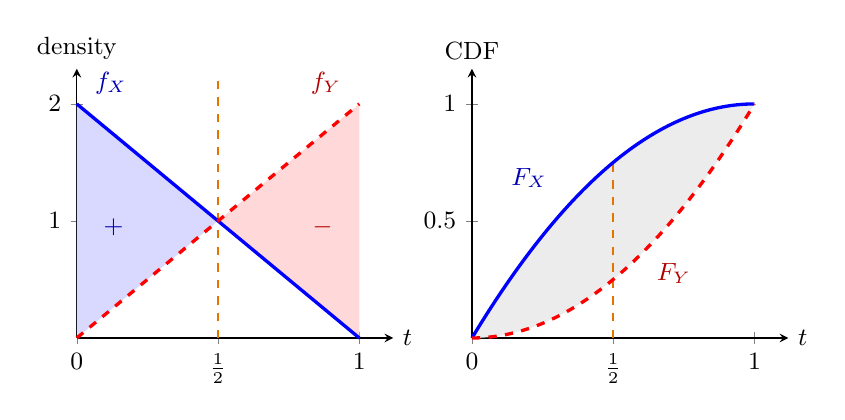
\begin{tikzpicture}[font=\small, >={Latex[length=2mm]}]
  \begin{axis}[name=left,
    axis lines=left, xmin=0, xmax=1.12, ymin=0, ymax=2.3,
    xtick={0,0.5,1}, xticklabels={$0$,$\tfrac12$,$1$}, ytick={1,2},
    xlabel={$t$}, ylabel={density},
    xlabel style={at={(axis description cs:1,0)}, anchor=west},
    ylabel style={rotate=-90, at={(axis description cs:0,1)}, anchor=south},
    width=5.6cm, height=5cm, clip=false]
    \addplot[fill=blue!15, draw=none] coordinates {(0,0) (0,2) (0.5,1) (0,0)};
    \addplot[fill=red!15, draw=none] coordinates {(0.5,1) (1,2) (1,0) (0.5,1)};
    \draw[orange!90!black, thick, dashed] (axis cs:0.5,0) -- (axis cs:0.5,2.2);
    \addplot[blue, very thick, domain=0:1] {2*(1-x)};
    \addplot[red, very thick, dashed, domain=0:1] {2*x};
    \node[blue!70!black, anchor=south west] at (axis cs:0.03,2.0) {$f_X$};
    \node[red!70!black, anchor=south east] at (axis cs:0.97,2.0) {$f_Y$};
    \node[blue!70!black] at (axis cs:0.13,0.95) {$+$};
    \node[red!70!black] at (axis cs:0.87,0.95) {$-$};
  \end{axis}
  \begin{axis}[at={(left.east)}, anchor=west, xshift=1.0cm,
    axis lines=left, xmin=0, xmax=1.12, ymin=0, ymax=1.15,
    xtick={0,0.5,1}, xticklabels={$0$,$\tfrac12$,$1$}, ytick={0.5,1},
    xlabel={$t$}, ylabel={CDF},
    xlabel style={at={(axis description cs:1,0)}, anchor=west},
    ylabel style={rotate=-90, at={(axis description cs:0,1)}, anchor=south},
    width=5.6cm, height=5cm, clip=false]
    \addplot[fill=gray!15, draw=none, domain=0:1, samples=60] {2*x-x^2} -- (axis cs:1,1) -- plot[domain=1:0, samples=60] ({\x},{\x^2}) -- cycle;
    \draw[orange!90!black, thick, dashed] (axis cs:0.5,0) -- (axis cs:0.5,0.75);
    \addplot[blue, very thick, domain=0:1, samples=60] {2*x-x^2};
    \addplot[red, very thick, dashed, domain=0:1, samples=60] {x^2};
    \node[blue!70!black, anchor=south east] at (axis cs:0.3,0.6) {$F_X$};
    \node[red!70!black, anchor=north west] at (axis cs:0.62,0.36) {$F_Y$};
  \end{axis}
\end{tikzpicture}
\end{document}
